\documentclass[../main.tex]{subfiles}

\begin{document}
\section{User Stories}\label{sec:userstories}

In this section, we will break down the user requirements into user stories, providing also some mockup crafted with balsamiq. Each user story represents a specific piece of functionality that adds value to our web-application, providing a clear, concise description of what needs to be implemented to better guide the development process. 

\textbf{User Registration:}
\begin{itemize}
  \item As a new user, I want to register inside the web application using my Facebook account in order to access the service.
  \begin{figure}[h]
	\centering
	\label{fig:pngegg}
	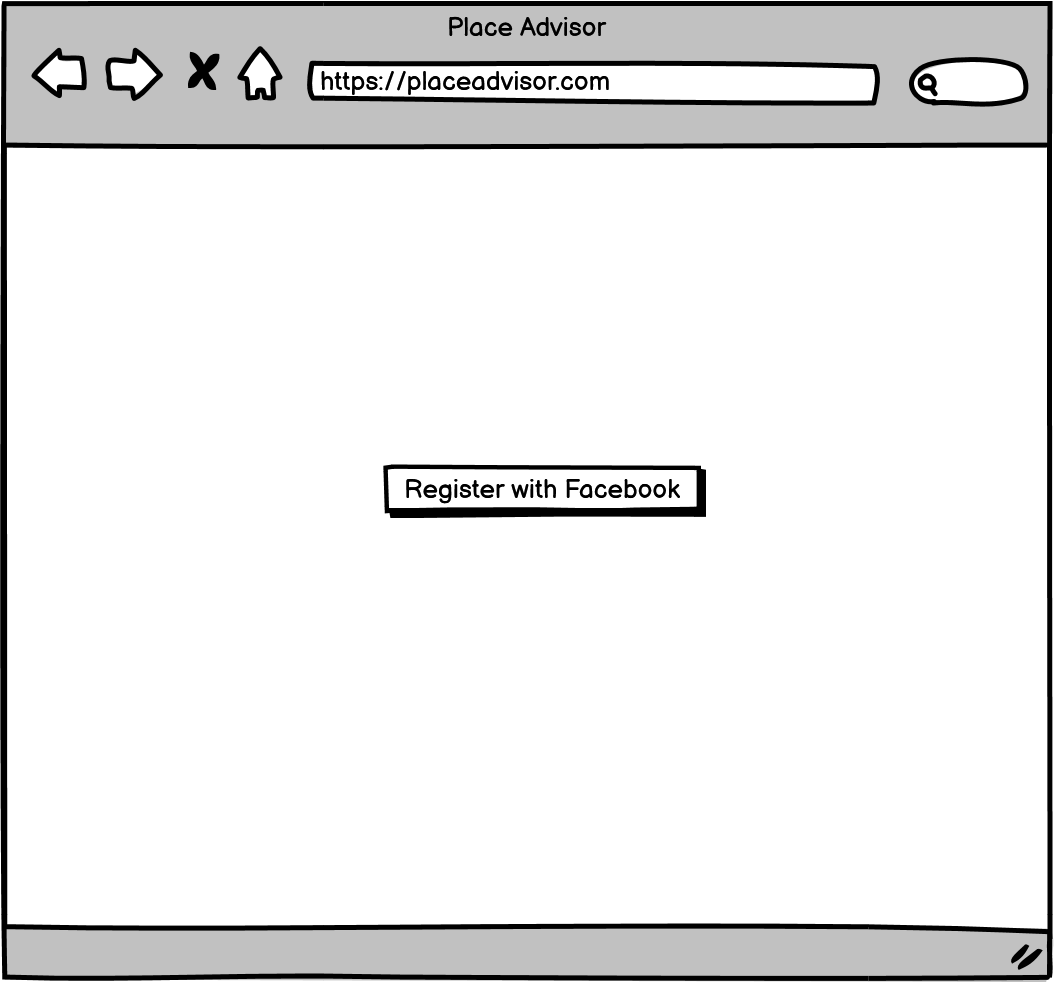
\includegraphics[width=0.5\linewidth]{../figures/mockup/US1.png}
  \end{figure}
  \item As a registered user, I want to be able to log in with my Facebook credentials to save time and avoid creating a new account.
  \begin{figure}[H]
	\centering
	\label{fig:pngegg}
	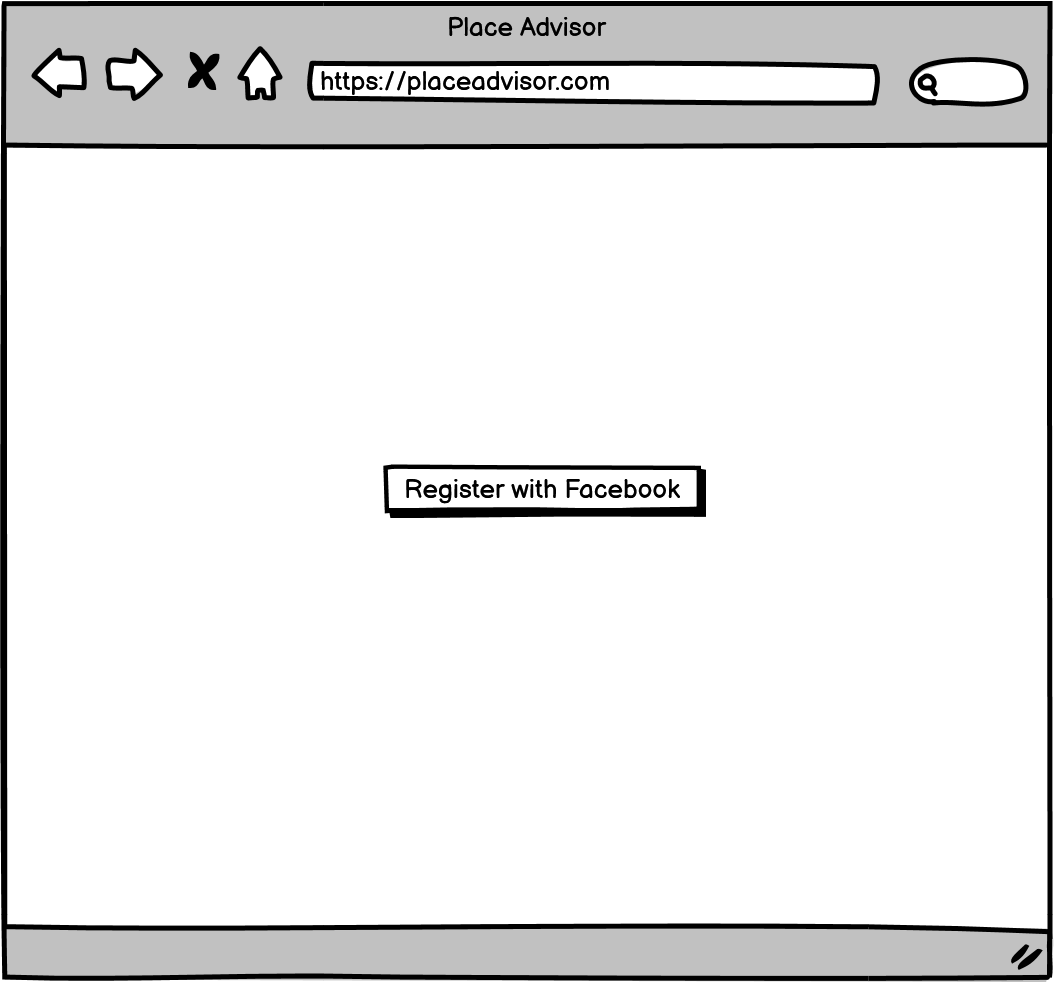
\includegraphics[width=0.5\linewidth]{../figures/mockup/US1.png}
  \end{figure}
  
\end{itemize}
\pagebreak
\textbf{Points of Interest Discovery:}
\begin{itemize}
  \item As a user, I want to search for points of interest in a specific area or city to discover new places to visit.
  \begin{figure*}[h]
\begin{multicols}{2}
    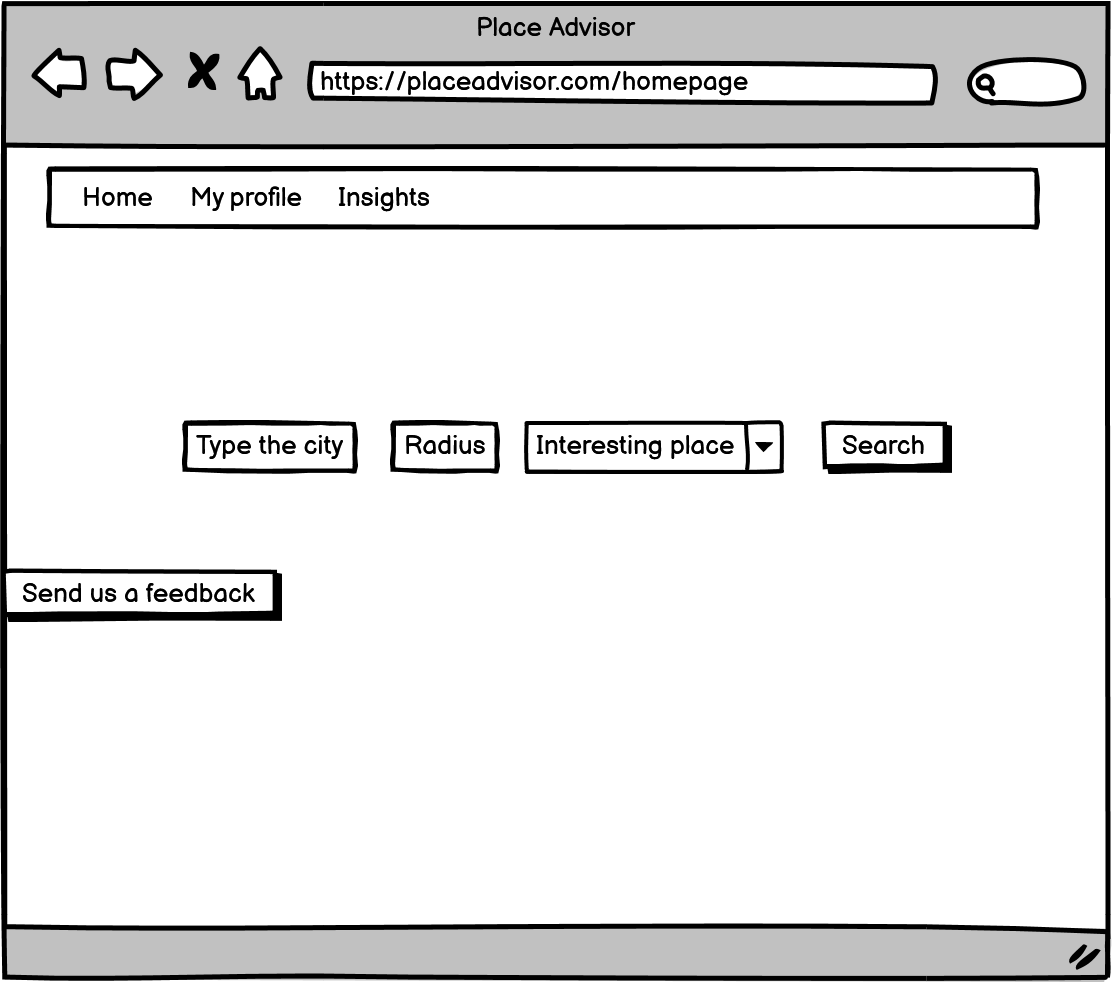
\includegraphics[width=\linewidth]{figures/mockup/US4.png}\par 
    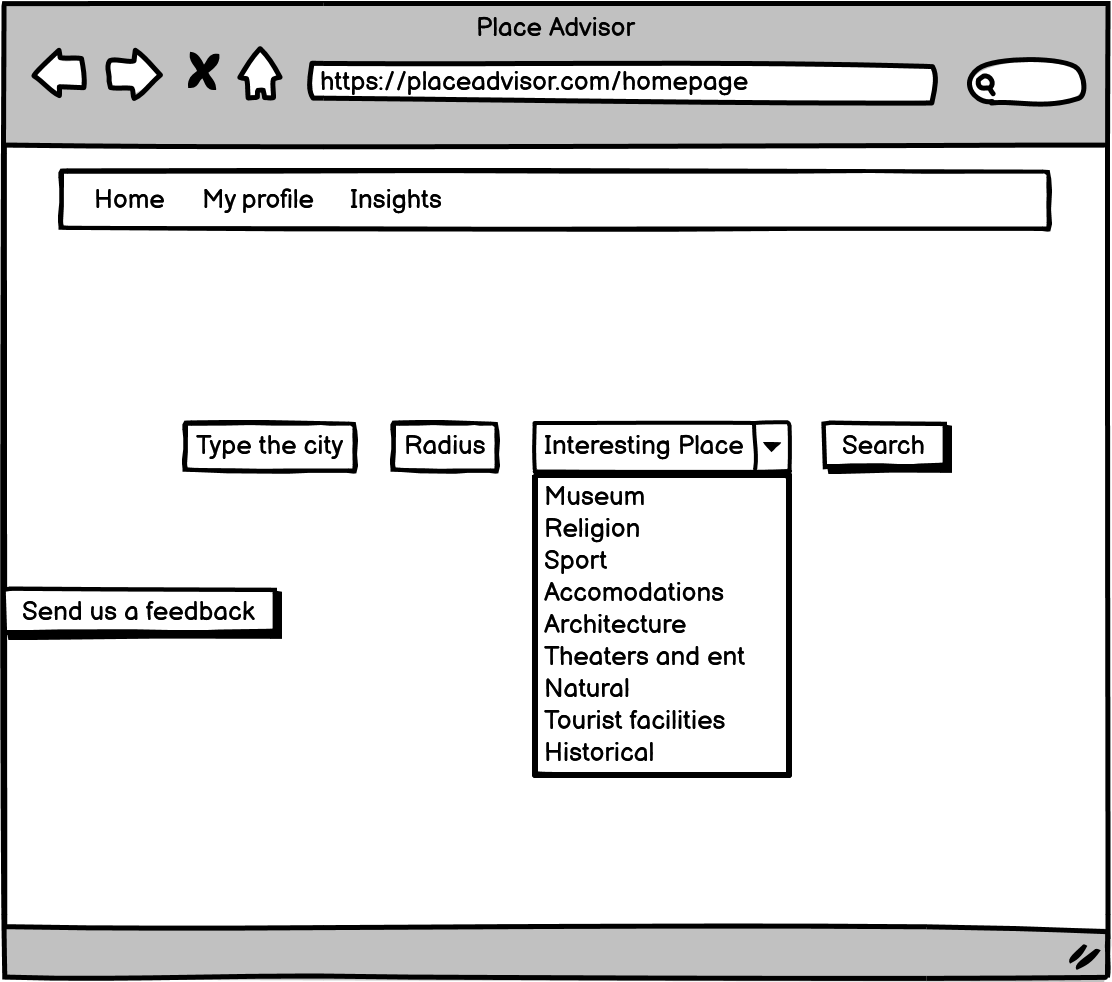
\includegraphics[width=\linewidth]{figures/mockup/US5.png}\par 
    \end{multicols}
\end{figure*}
  
  \item As a user, I want to view detailed information about a point of interest, including its address, historical facts, and other relevant details, in order to make informed decisions about visiting it.
  \item As a user, I want to read reviews and ratings of points of interest from other users to get insights into their experiences.
  \item As a user, I want to leave my own reviews and ratings for points of interest to share my opinions and help others make informed choices.
  \begin{figure}[H]
	\centering
	\label{fig:pngegg}
	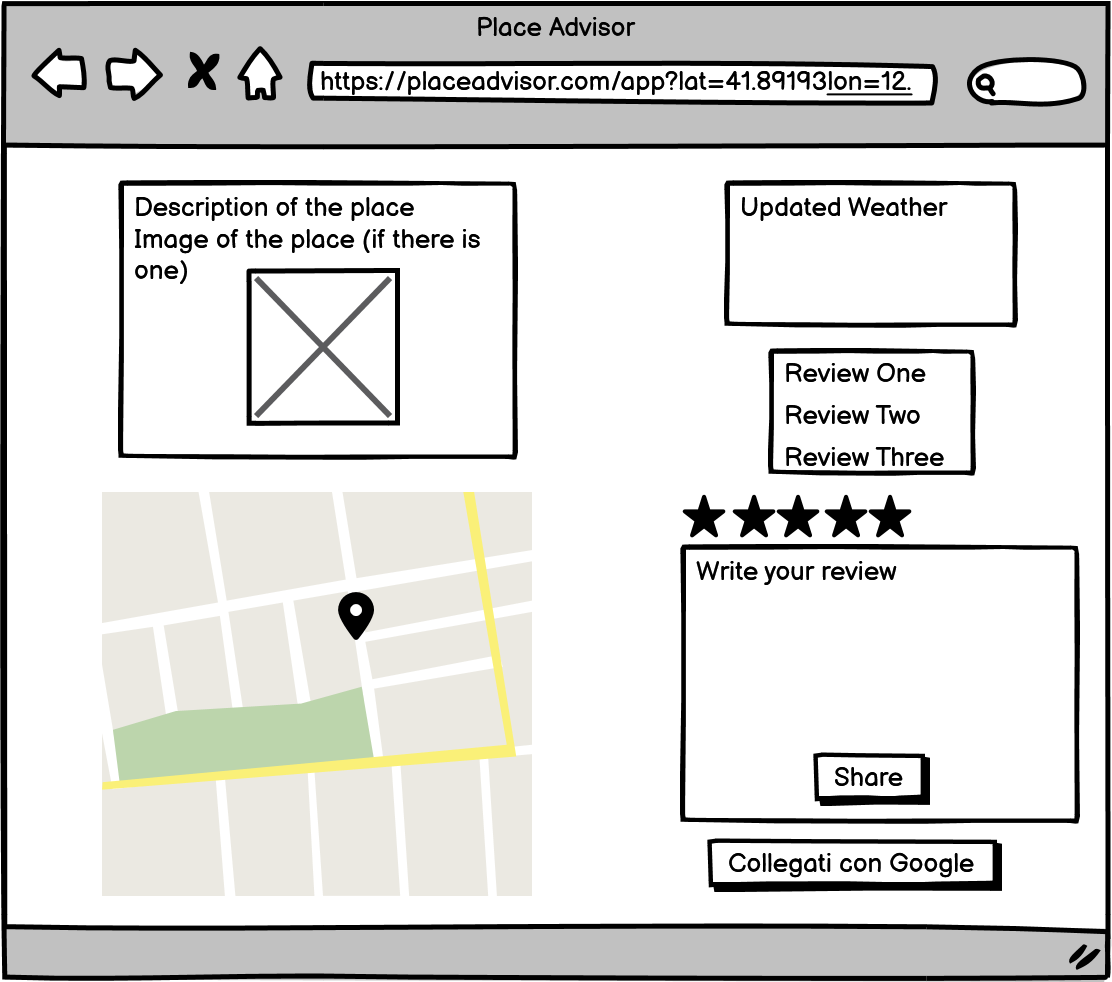
\includegraphics[width=0.5\linewidth]{../figures/mockup/US7.png}
  \end{figure}
\end{itemize}
\pagebreak
\textbf{Photo Integration and User Profiles:}
\begin{itemize}
  \item As a user, I want to login with Google and upload and attach photos to points of interest to visually share my experiences with others.
  \begin{figure}[H]
	\centering
	\label{fig:pngegg}
	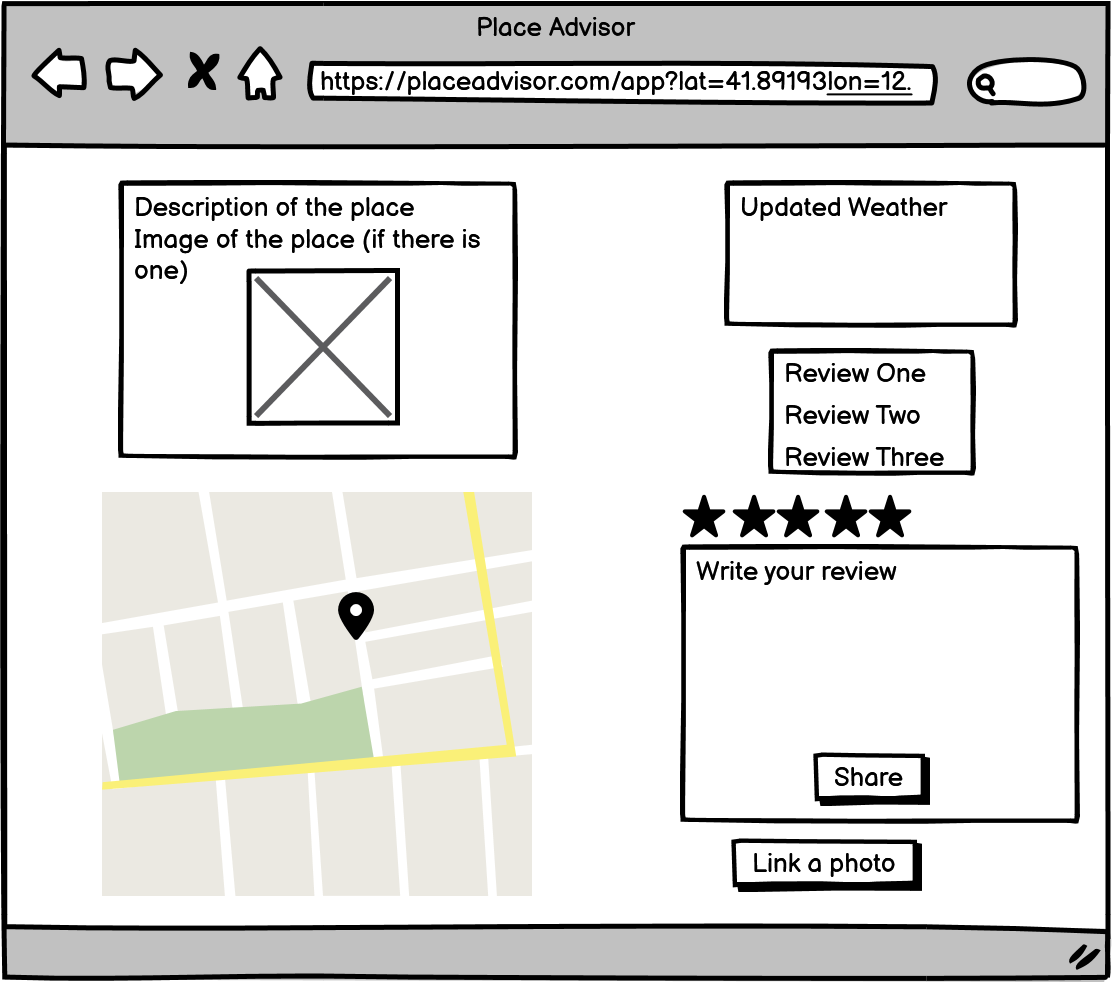
\includegraphics[width=0.5\linewidth]{../figures/mockup/US7 copy.png}
  \end{figure}
  \item As a user, I want to access my user profile page to see all my details and view the list of the feedbacks and reviews I have submitted.
    \begin{figure*}[h]
\begin{multicols}{2}
    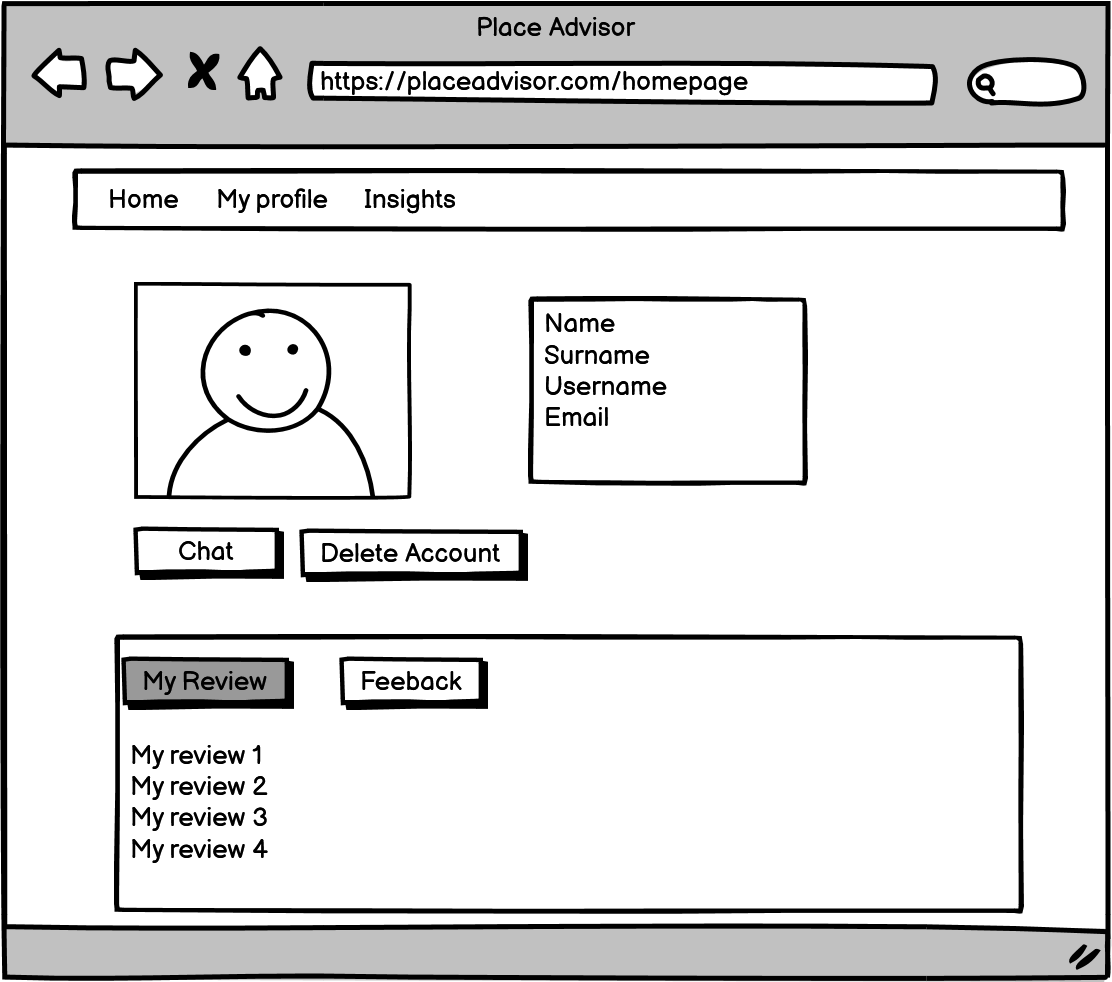
\includegraphics[width=\linewidth]{../figures/mockup/US8.png}\par 
    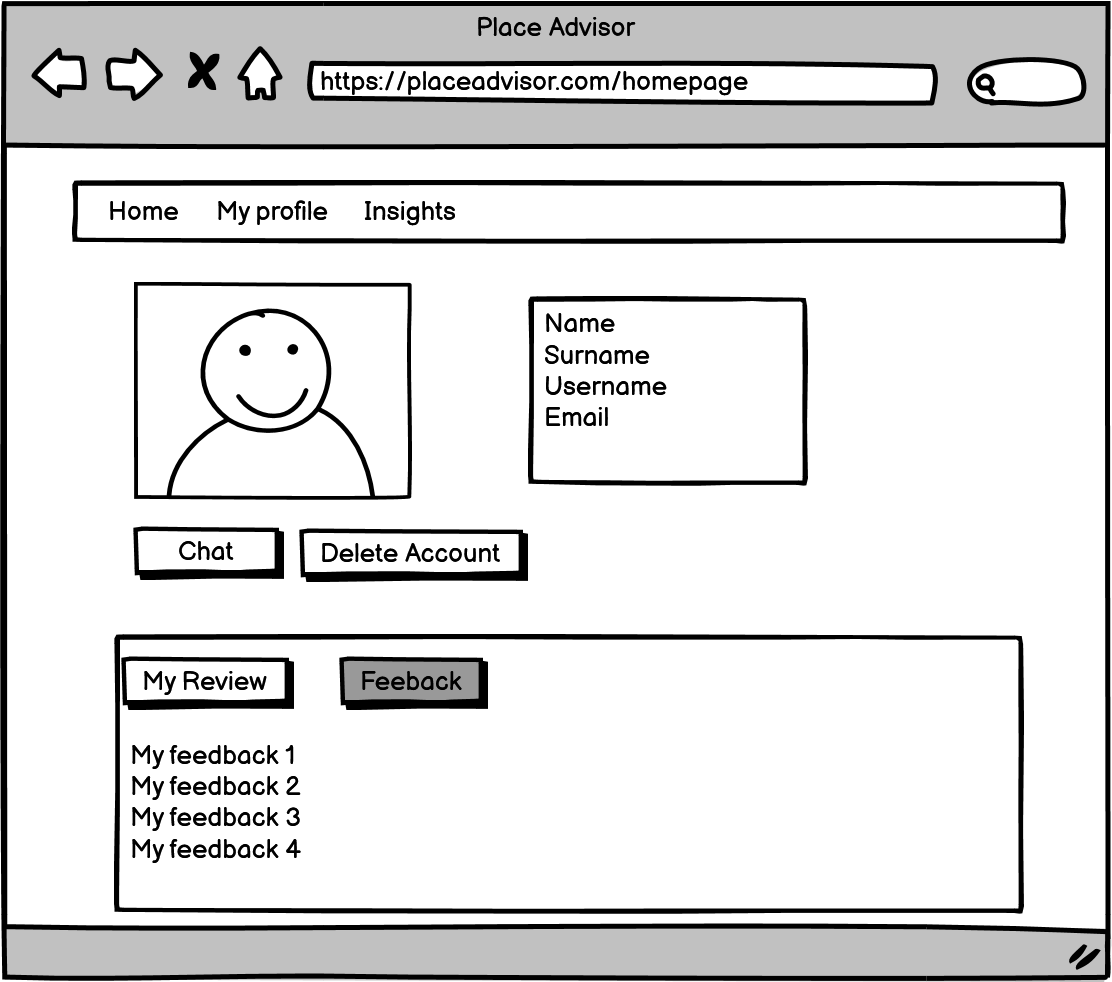
\includegraphics[width=\linewidth]{../figures/mockup/US8 copy.png}\par 
    \end{multicols}
\end{figure*}
  
\end{itemize}

\textbf{User Account Management:}
\begin{itemize}
  \item As a registered user, I want to have the ability to log out of my PlaceAdvisor account and delete my account to ensure the security and privacy of my data and to have control over my account status.
\end{itemize}

\pagebreak

\textbf{User Feedback and Suggestions:}
\begin{itemize}
  \item As a user, I want to provide feedback or suggestions about the app's features and functionality to improve the quality of service.
\end{itemize}

\begin{figure*}[h!]
  \begin{multicols}{2}
    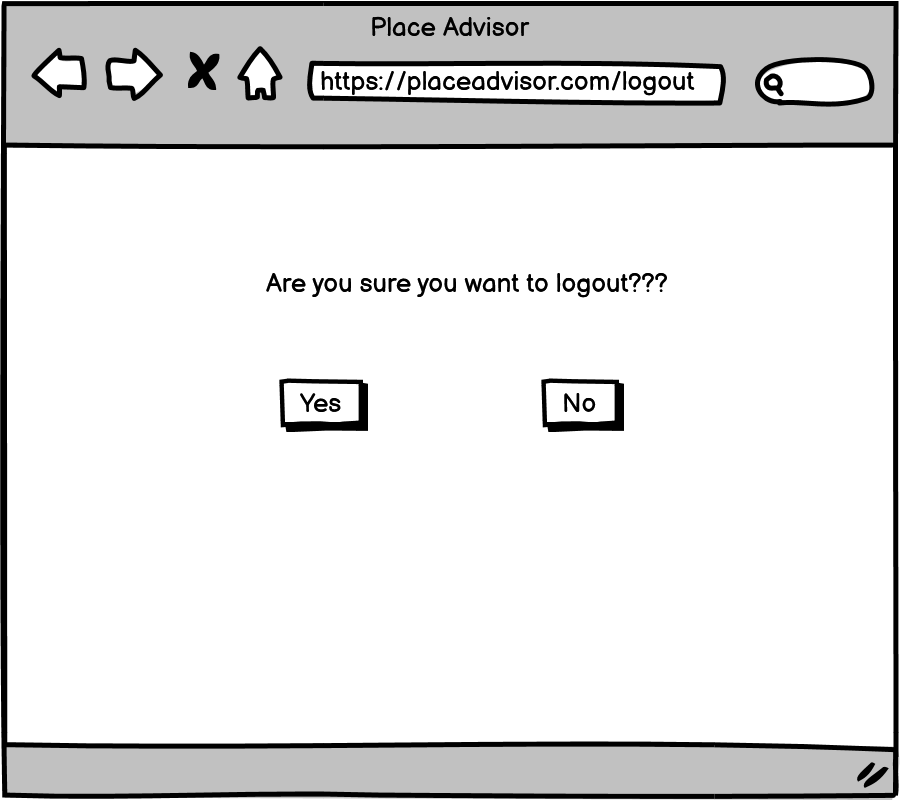
\includegraphics[width=\linewidth]{../figures/mockup/New Wireframe 1.png}\par 
    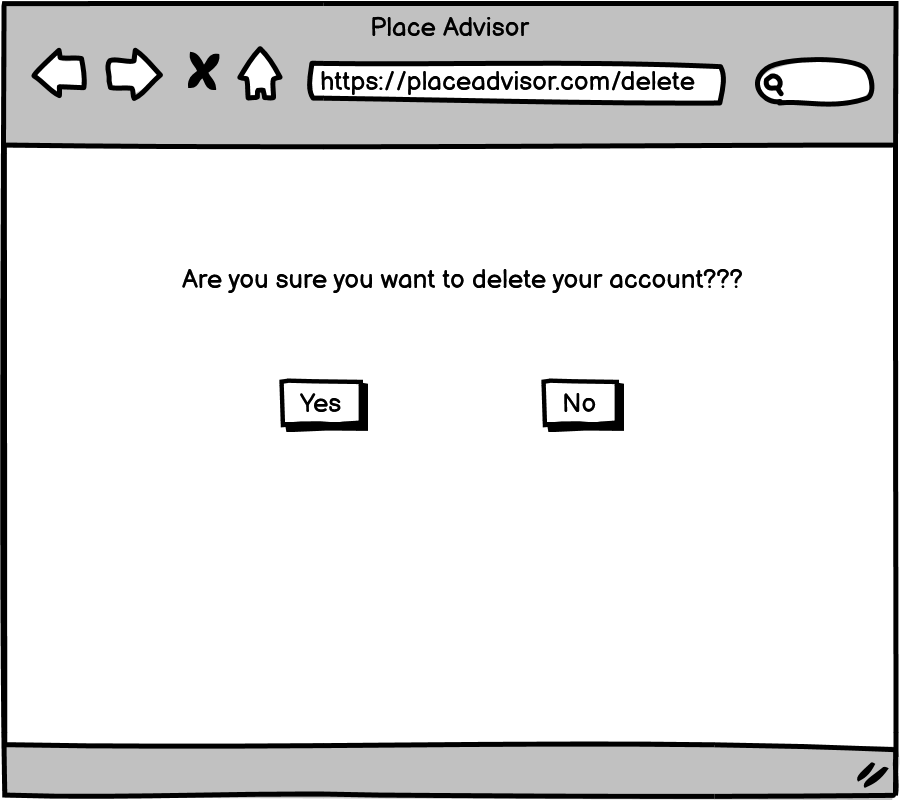
\includegraphics[width=\linewidth]{../figures/mockup/New Wireframe 1 copy.png}\par 
  \end{multicols}
\end{figure*}

\textbf{Analytics and Insights:}
\begin{itemize}
  \item As a user, I want access to analytics and insights about points of interest to gain a better understanding of popular destinations and trends.
  \begin{figure}[H]
	\centering
	\label{fig:pngegg}
	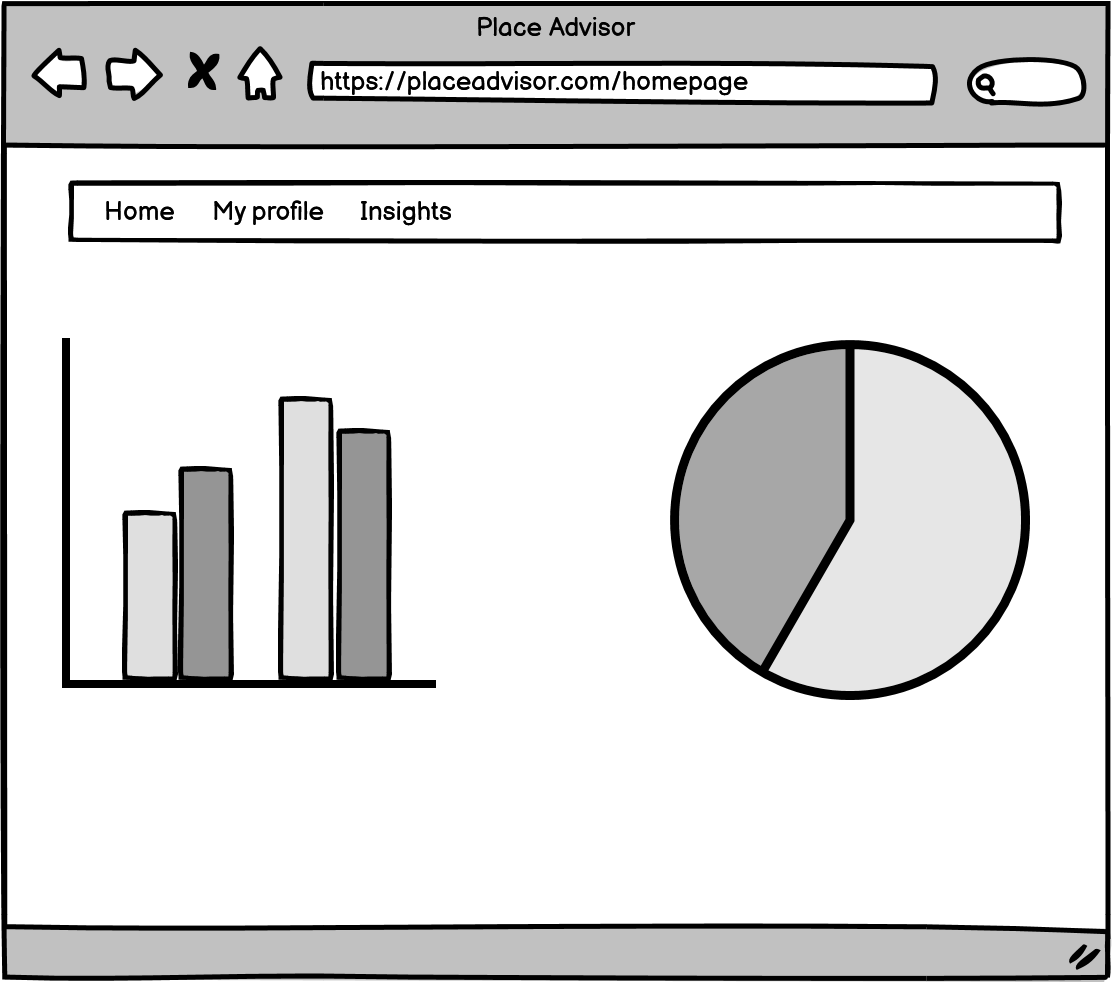
\includegraphics[width=0.5\linewidth]{../figures/mockup/US9.png}
  \end{figure}
\end{itemize}

\pagebreak

\textbf{Customer Support:}
\begin{itemize}
  \item As a Customer Care representative, I want to log in inside the web application to find if there are some users that need help.
  \begin{figure*}[h]
\begin{multicols}{2}
    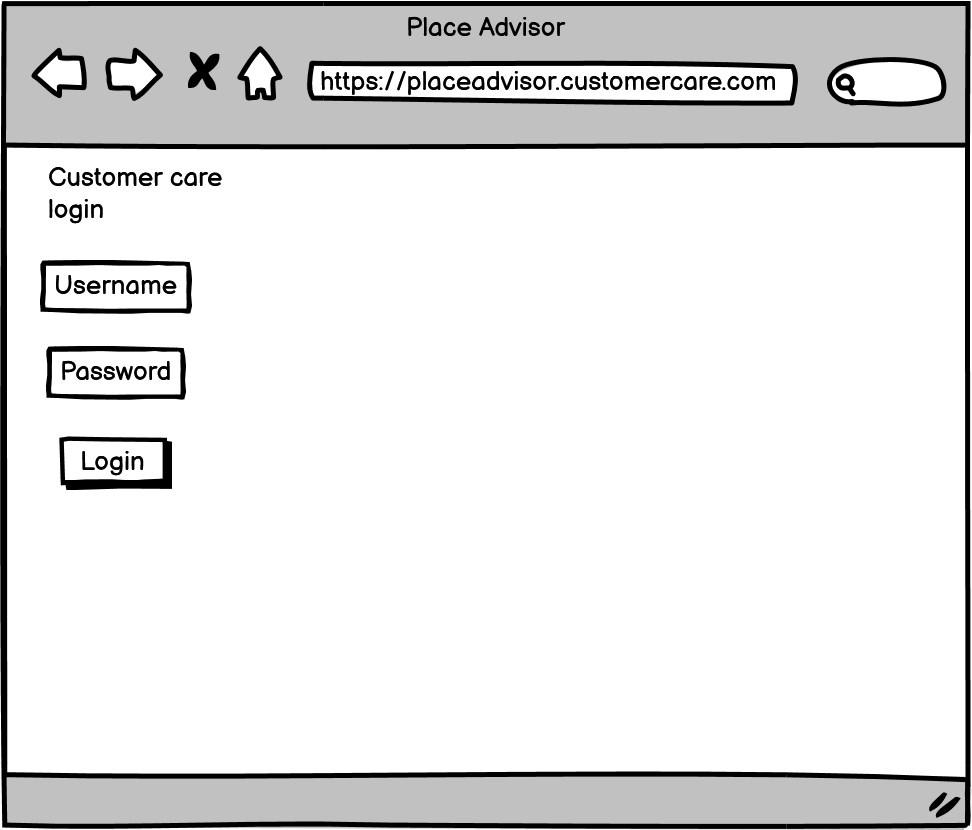
\includegraphics[width=\linewidth]{../figures/mockup/US10 copy.png}\par 
    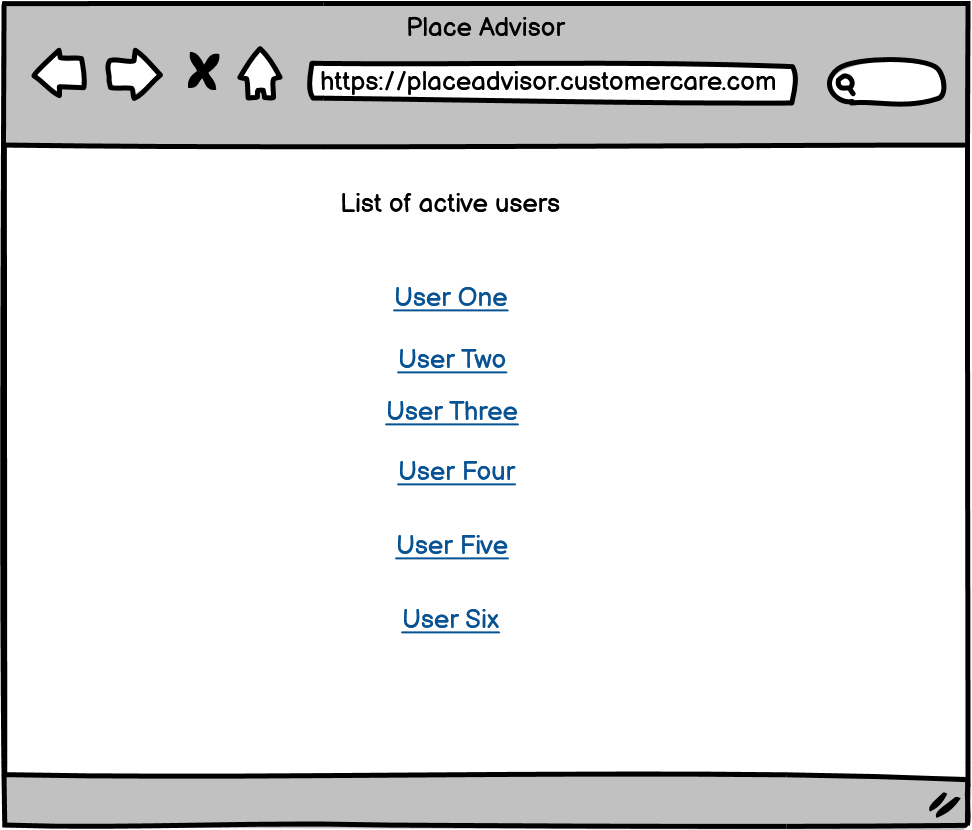
\includegraphics[width=\linewidth]{../figures/mockup/US10 copy 2.png}\par 
    \end{multicols}
\end{figure*}
  \item As a user, I want to initiate a real-time chat with support representatives to get assistance with app-related issues.
  \begin{figure*}[h]
\begin{multicols}{2}
    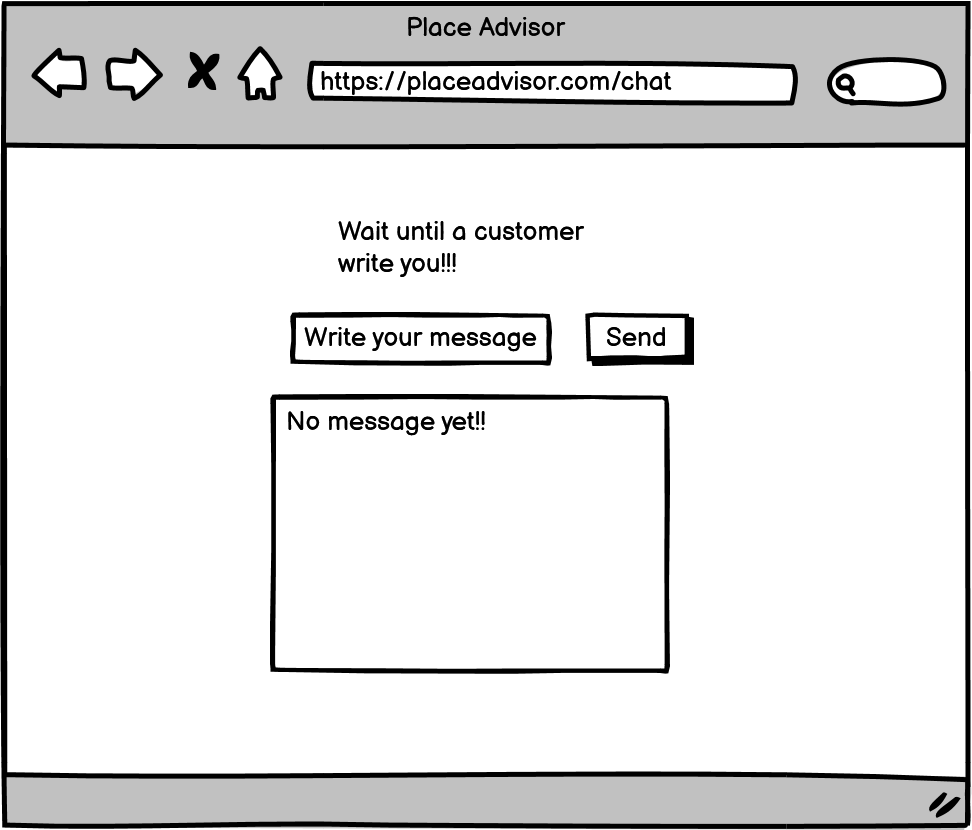
\includegraphics[width=\linewidth]{../figures/mockup/US10.png}\par 
    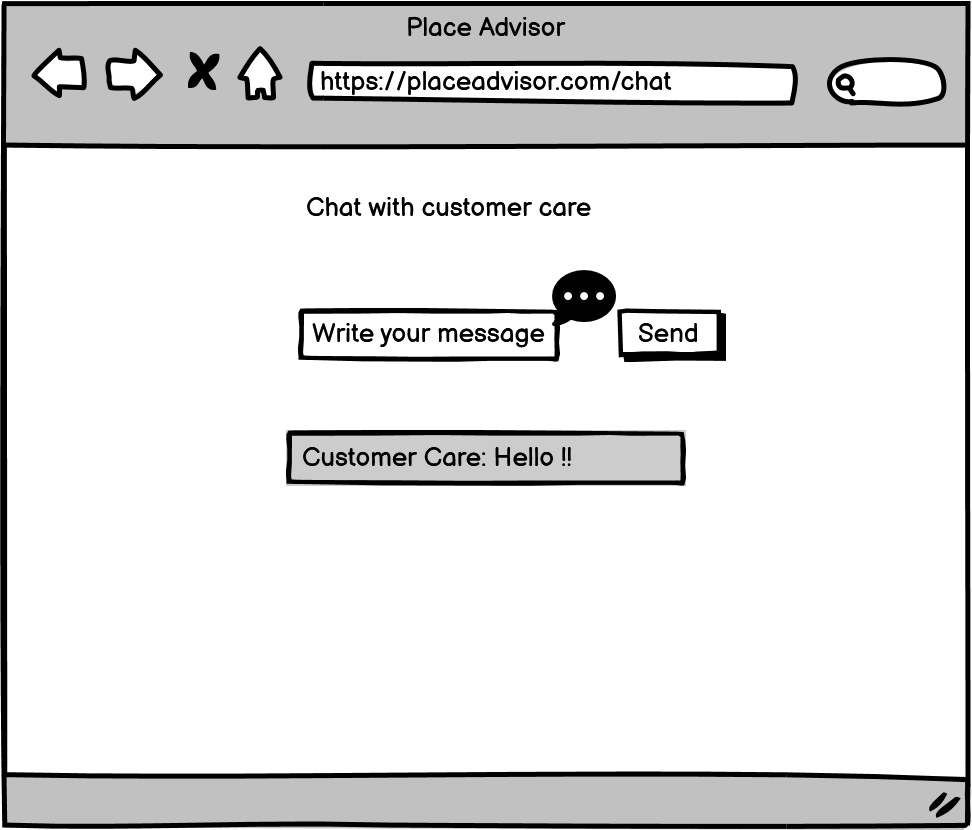
\includegraphics[width=\linewidth]{../figures/mockup/US12.png}\par 
    \end{multicols}
\end{figure*}
\pagebreak
  \item As Customer Care, I want to chat with users of the web application to assist the users and respond to their questions.
  \begin{figure}[H]
	\centering
	\label{fig:pngegg}
	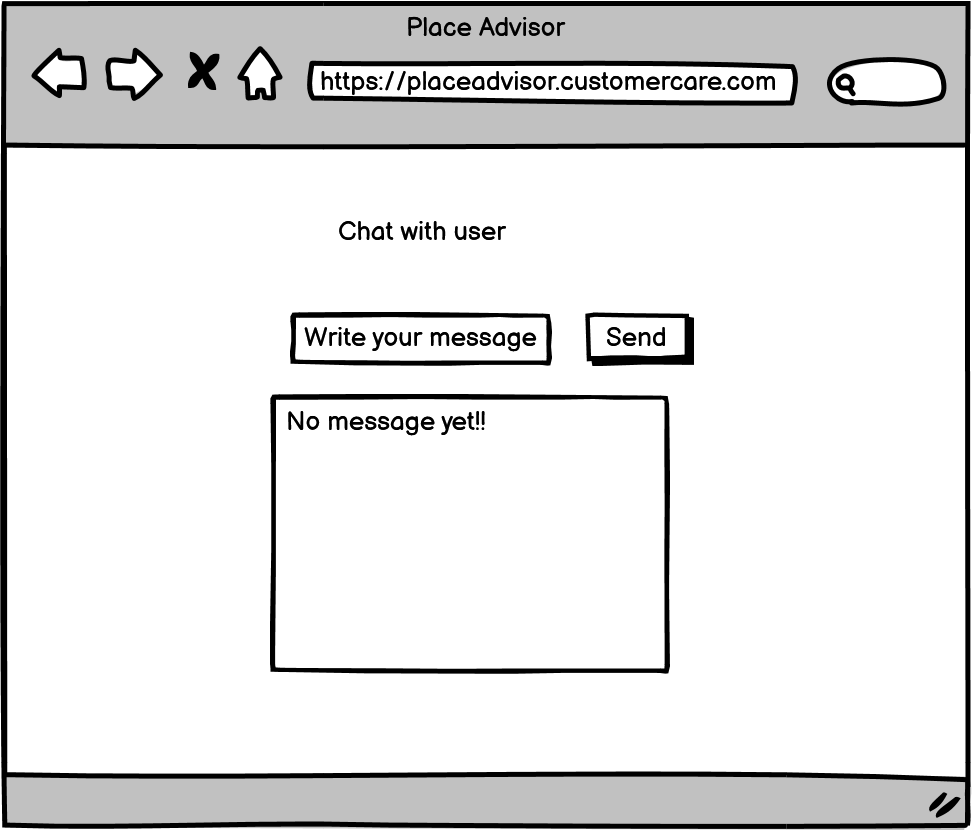
\includegraphics[width=0.5\linewidth]{../figures/mockup/US10 copy 3.png}
  \end{figure}
\end{itemize}


\textbf{API Documentation and Security:}
\begin{itemize}
  \item As a User/Developer, I want to access API documentation to understand how to use and integrate with the PlaceAdvisor API effectively.
  \item As a user, I want my authentication session to persist securely to have a seamless experience and not re-login frequently.
  \item As a security-conscious user, I want to access PlaceAdvisor via a secure HTTPS connection to protect my data and ensure secure communication.
\end{itemize}

\textbf{Infrastructure and Aesthetics:}
\begin{itemize}
  \item As a developer, I want to integrate Docker Compose to simplify the deployment and scaling of our application components and ensure consistent development and production environments.
  \item As a user, I want a dashboard with Kibana and Elasticsearch for insights into user and POI data to make data-driven decisions and gain valuable insights.
  \item As a user, I want the pages of the PlaceAdvisor website to have an improved aesthetic design to have a visually pleasing and engaging experience while using the platform.
\end{itemize}




\end{document}


\begin{figure}[h]
	\centering
	\caption{Registration through Facebook}
	\label{fig:pngegg}
	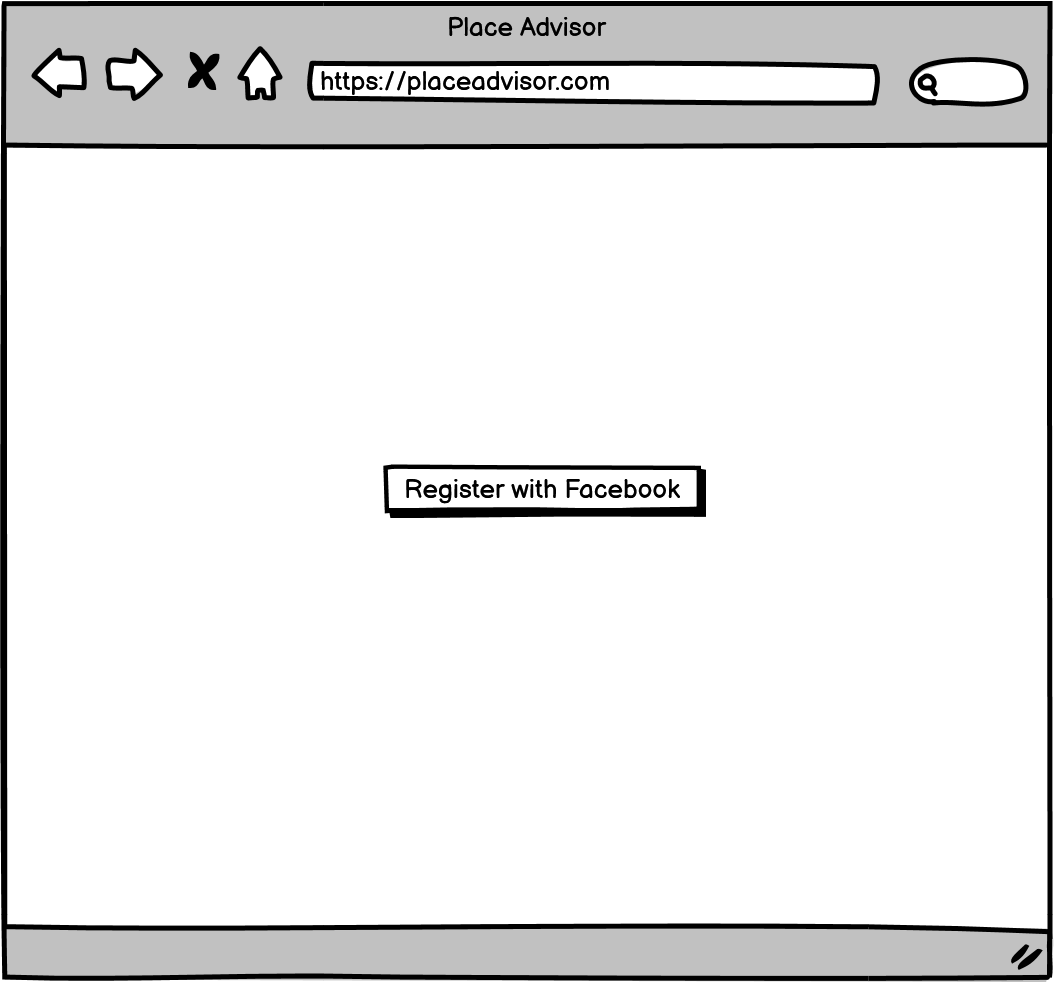
\includegraphics[width=0.7\linewidth]{../figures/mockup/US1.png}
\end{figure}